The project is designed to be deployed in the cloud, specifically in a Kubernetes as a Service (KaaS) solution. To evaluate the cost of different cloud providers, an open-sourced cost calculator \cite{managed_kubernetes_pricing} was used. The results for the most popular cloud providers, including Amazon Web Services (AWS), Azure (AKS), Google Cloud (GKE), and Digital Ocean (DO) can be seen in the plot below.

\begin{figure}[H]
    \centering
    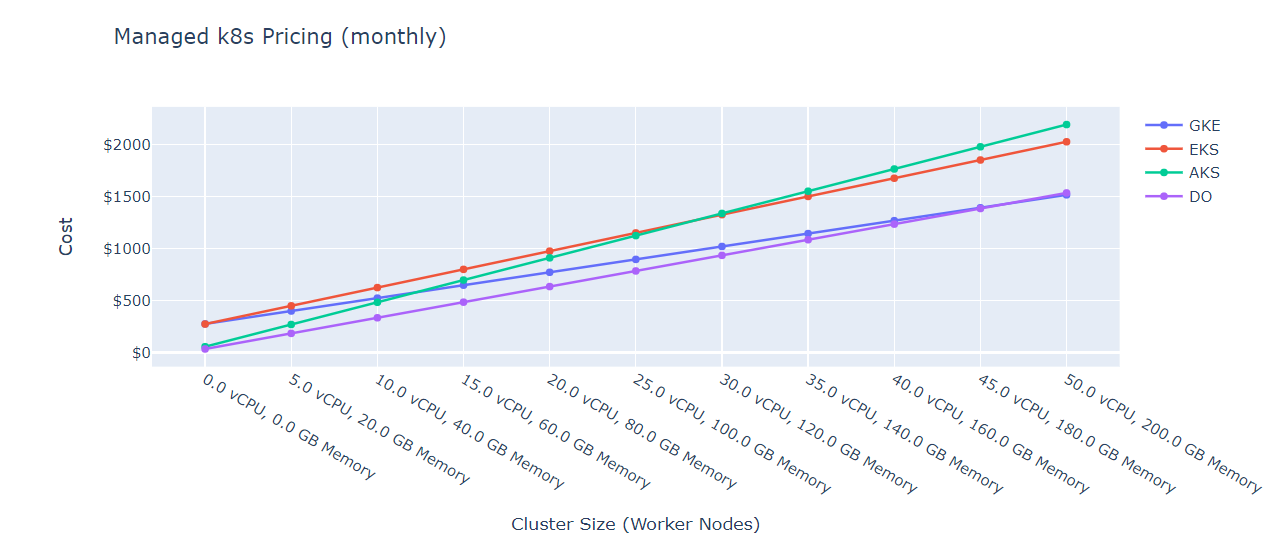
\includegraphics[width=\textwidth]{pictures/k8s_cost.png}
    \caption{ Managed Kubernetes cost }
    \label{fig:k8s_cost}
\end{figure}

For small-scale projects, Digital Ocean and Azure are the most cost-effective options as they do not charge for the compute used for the control plane. For large-scale projects, Google Cloud is the most affordable.

Two cloud providers, Microsoft Azure and Okteto Cloud, were evaluated for this implementation. Both providers offer Kubernetes as a Service, but they have adopted different approaches.

In Azure, the Kubernetes cluster is created and then primarily managed by the user. This approach is more difficult to maintain, but also more flexible as the cluster can be easily scaled and extended.

In contrast, Okteto Cloud has adopted a different approach, focusing on creating a development environment that is not typically production-ready. In the free tier, Okteto Cloud provides a namespace in a cluster that is fully managed by Okteto, with the possibility of deploying up to 10 pods with limitations as specified below.
\begin{itemize}
    \item Namespaces: 5
    \item Pods: 10
    \item CPU: 1 / pod
    \item Memory: 3Gi / pod
    \item Storage: 5Gi
\end{itemize}

The result of the comparison between Azure and Okteto Cloud is that Okteto Cloud is better suited for development purposes while Azure is more suitable for productization. Okteto Cloud is focused on creating development environments that are not typically production-ready, and it's also free, it's limited to 10 pods and not suitable for large projects. On the other hand, Azure provides more flexibility and scalability options, but it's harder to maintain and it's more expensive. It's a better fit for large projects and production-ready systems. Based on this evaluation, Okteto Cloud will be used for the implementation of this project, as it provides an appropriate development environment and is cost-effective.